\documentclass[11pt]{article}
\usepackage[a4paper,margin=2.2cm]{geometry}
\usepackage{amsmath,amssymb}
\usepackage{booktabs}
\usepackage{graphicx}
\usepackage{float}
\usepackage{caption}
\usepackage{enumitem}
\usepackage{xcolor}
\usepackage{microtype}
\usepackage[hidelinks]{hyperref}
\setlist{nosep,leftmargin=1.4em}
\setlength{\parskip}{4pt}
\setlength{\parindent}{0pt}
\captionsetup{font=small,labelfont=bf}
\newcommand{\ms}{\,m/s$^2$}
\newcommand{\mss}{\,(m/s$^2$)$^2$}
\newcommand{\todo}[1]{\textcolor{red}{[#1]}}
\makeatletter
\newcommand{\inputrows}[1]{\@@input #1 }   % expandable input for generated table rows
\makeatother
\def\UrlBreaks{\do\/\do\_\do\-\do\.}      % let long paths wrap

\title{AI651 -- Deep Learning for Space, Time and Graphs\\[2pt] \large Assignment 1: Forecasting across heterogeneous sensors, and an Autoformer leaderboard}
\author{Muteeullah Baig \quad 25280036\\[2pt]
\small Code: \url{https://github.com/MuteeullahBaig/AI651-PA1}}
\date{2 October 2026}

\begin{document}
\maketitle

\section*{Task 1 -- Forecasting across heterogeneous sensors}

\paragraph{Run.} Every number and figure below comes from one fresh top-to-bottom execution of
\path{task1/Assignment1.ipynb} with \texttt{PA1\_PRESET=full}, data seed 0 and model seed 0, on an RTX~4070 Laptop GPU. The run took 280\,s, and every notebook check passed. ``Established'' means stations 1--3 and ``held-out'' means station~4. Each claim below names its population and its split (training, validation or test).

\paragraph{Implementations.}
\begin{itemize}
  \item \textbf{\texttt{RawAttentionForecaster.forward}} embeds the context ($[B,1,L]\!\to\![B,d,L]$), transposes back and adds the learned position table. It then applies both encoder blocks and the final LayerNorm, flattens $[B,L,d]$, and maps it to $[B,H]$ with the forecast head.
  \item \textbf{\texttt{SeriesDecomposition.forward}} replicates the first and last values $\lfloor m/2\rfloor$ times along time, averages with a stride-1 \texttt{avg\_pool1d} over time for every channel, and returns $(x-T,\,T)$.
  \item \textbf{\texttt{aggregate\_delays}} builds, per example, the source index $(t-\tau_j)\bmod L$, gathers the $K$ shifted copies of the values with \texttt{torch.gather}, and sums them weighted by $\alpha_j$. It is fully vectorized and differentiable in both values and weights.
\end{itemize}

% ---------------------------------------------------------------------------------------------
\subsection*{Response 1A -- predicted, measured and revised ordering}

\textbf{Prediction} (recorded in \path{task1/predictions_before_running.md} before any cell ran; drafted with AI assistance, see the appendix):
established, period-routed ridge $<$ Raw Attention $<$ shared ridge $\approx$ sensor-specific ridge;
held-out, period-routed ridge $<$ Raw Attention $<$ shared ridge (sensor-specific ridge unavailable).

\begin{table}[H]\centering\small
\caption{Output 1.1, validation. RMSE in \ms, MSE in \mss. Columns A, B and C give RMSE by product.}
\resizebox{\linewidth}{!}{\begin{tabular}{lrrrrrrrrrrr}
\toprule
 & \multicolumn{5}{c}{Established stations 1--3} & \multicolumn{5}{c}{Held-out station 4} & \\
\cmidrule(lr){2-6}\cmidrule(lr){7-11}
Model & RMSE & MSE & A & B & C & RMSE & MSE & A & B & C & Params \\
\midrule
Shared ridge          & 0.767 & 0.588 & 0.805 & 0.854 & 0.621 & 0.876 & 0.767 & 0.909 & 0.982 & 0.713 & 4{,}608 \\
Sensor-specific ridge & 0.768 & 0.590 & 0.804 & 0.852 & 0.630 & --    & --    & --    & --    & --    & 13{,}824 \\
Period-routed ridge   & \textbf{0.166} & \textbf{0.028} & 0.181 & 0.164 & 0.152 & \textbf{0.173} & \textbf{0.030} & 0.184 & 0.182 & 0.150 & 59{,}904 \\
Raw Attention         & 0.408 & 0.166 & 0.376 & 0.434 & 0.410 & 0.577 & 0.333 & 0.565 & 0.548 & 0.616 & 368{,}368 \\
\bottomrule
\end{tabular}}
\end{table}

\textbf{Measured} (validation). The ordering holds in both populations and for every product.
\begin{itemize}
  \item \textbf{Period routing is far ahead of everything else.} On established stations its RMSE is 4.6$\times$ lower than shared ridge (0.166 vs 0.767) and 2.5$\times$ lower than Raw Attention (0.408). Raw Attention halves shared ridge's error ($-$47\%).
  \item \textbf{Station identity buys nothing.} On established stations, sensor-specific ridge equals shared ridge (0.768 vs 0.767) with three times the parameters.
  \item \textbf{Moving to station~4 costs very different amounts.} From established to held-out RMSE, period-routed ridge loses 4\% (0.166$\to$0.173), shared ridge 14\% (0.767$\to$0.876) and Raw Attention 41\% (0.408$\to$0.577).
  \item \textbf{Product effects.} Routed ridge is nearly flat across products in both populations (0.150--0.184). The unconditioned ridges are worst on Product~B and best on Product~C in both populations. Raw Attention has no consistent product ranking: established stations are worst on B (0.434), station~4 worst on C (0.616).
\end{itemize}

\textbf{Revision.} The ordering stands. I underestimated two magnitudes: routing's margin over Raw Attention, and Raw Attention's 41\% loss on station~4. I had also expected no station-4 loss for the linear shared map.

\textbf{Explanation by assumptions.}
\begin{itemize}
  \item \textbf{Shared ridge} applies one operator to every pace from 14 to 36 samples, so least squares settles on a compromise.
  \item \textbf{Sensor-specific ridge} conditions on a variable that does not determine the pace, since every station runs every pace. It therefore makes the same compromise.
  \item \textbf{Period-routed ridge} conditions on the variable that actually changes. Within a 1.5-sample band a linear map is nearly ideal for a sinusoid plus a smooth ramp. It does not use station identity, so it transfers almost unchanged to station~4.
  \item \textbf{Raw Attention} can build a context-dependent rule, but it must learn it from about 1{,}950 drift-dominated training windows. Its features are tied to the training stations' amplitudes and offsets, which is consistent with its large validation loss on station~4.
  \item \textbf{Shared ridge's 14\% station-4 loss is proportionate.} Its compromise error is a fixed fraction of the vibration it mis-predicts. Station~4 vibrates at 2.15\ms, against a mean of 1.88\ms\ for stations 1--3, a ratio of 1.14, which matches its validation error ratio $0.876/0.767 = 1.14$.
\end{itemize}

% ---------------------------------------------------------------------------------------------
\subsection*{Response 1B -- why the rule must depend on the context}

\begin{figure}[H]\centering
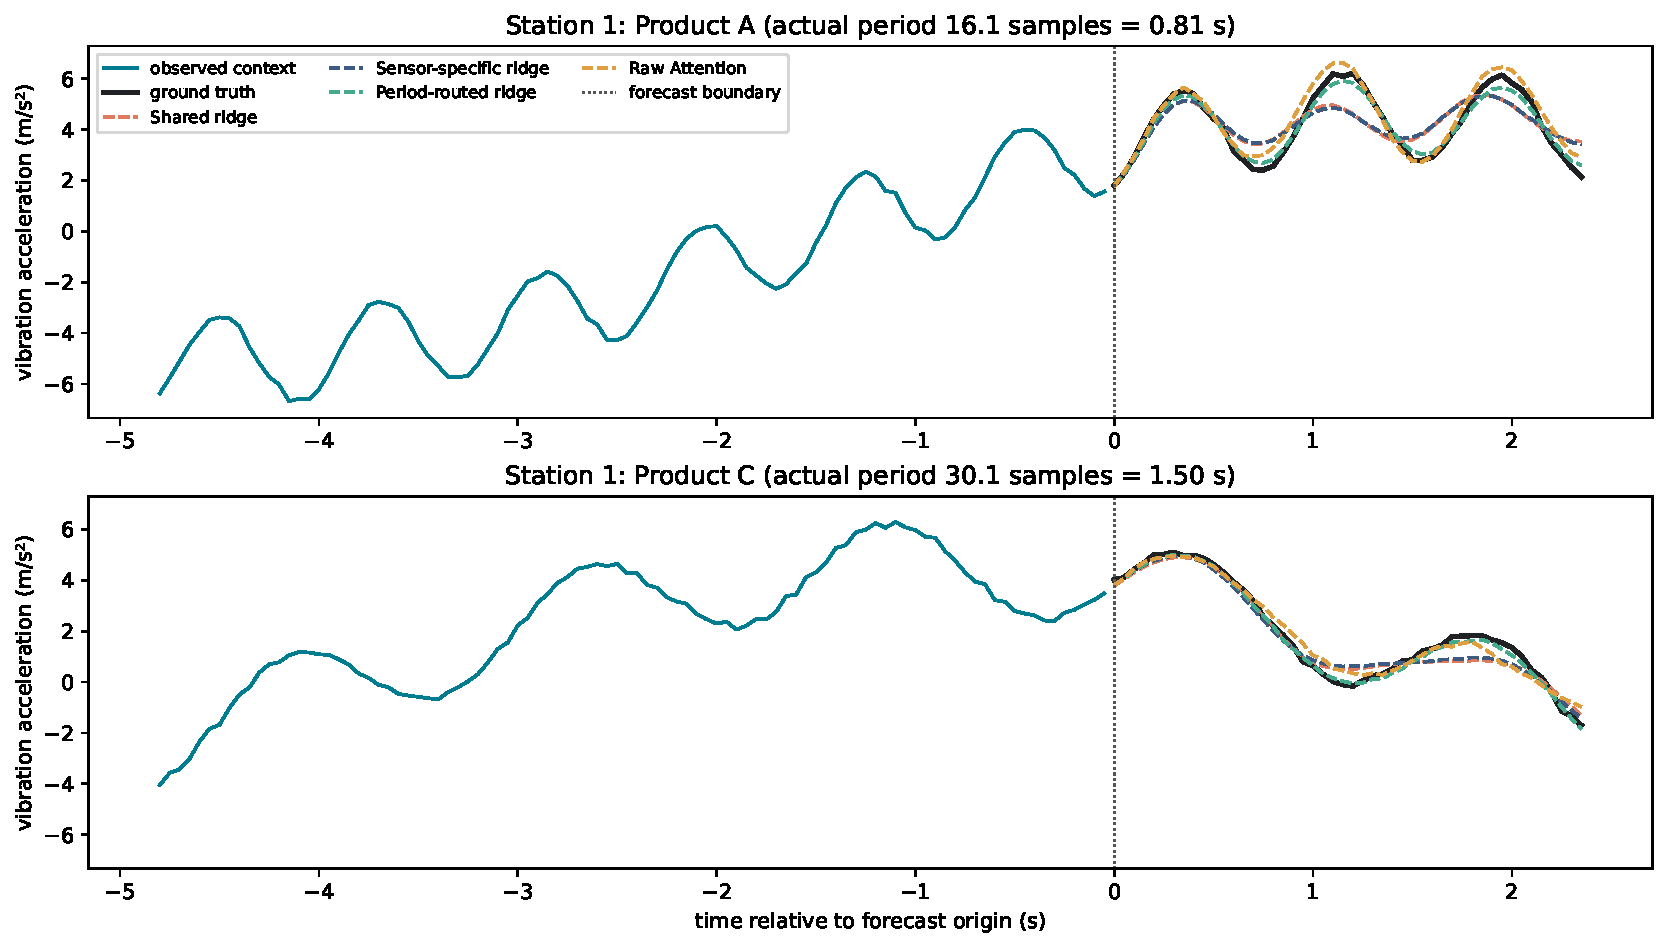
\includegraphics[width=0.83\linewidth]{figures/task1/1.2-1.pdf}
\caption{Output 1.2: station 1 (established) in a Product A validation run ($P=16.1$) and a Product C validation run ($P=30.1$).}
\end{figure}

\textbf{The compromise in the forecast} (station 1, validation). In the Product A window, shared and sensor-specific ridge get the first half-cycle's phase roughly right, but the oscillation then \emph{shrinks}. Predicted peaks reach about 4.9\ms\ against a true 6.2\ms, and predicted troughs sit near 3.5\ms\ against a true 2.4\ms. Their window RMSE is 0.78, against 0.23 for routed ridge. In the Product C window, the second, slower bump is flattened into a plateau (window RMSE 0.45 against 0.15).

A single $\hat W$ in equation (8) has no variable that selects the phase advance per step, so least squares averages the continuations of incompatible paces. Under squared error, the best response to phase uncertainty is the conditional mean, and an average of out-of-phase sinusoids has a smaller amplitude. That is the damping we see.

\begin{figure}[H]\centering
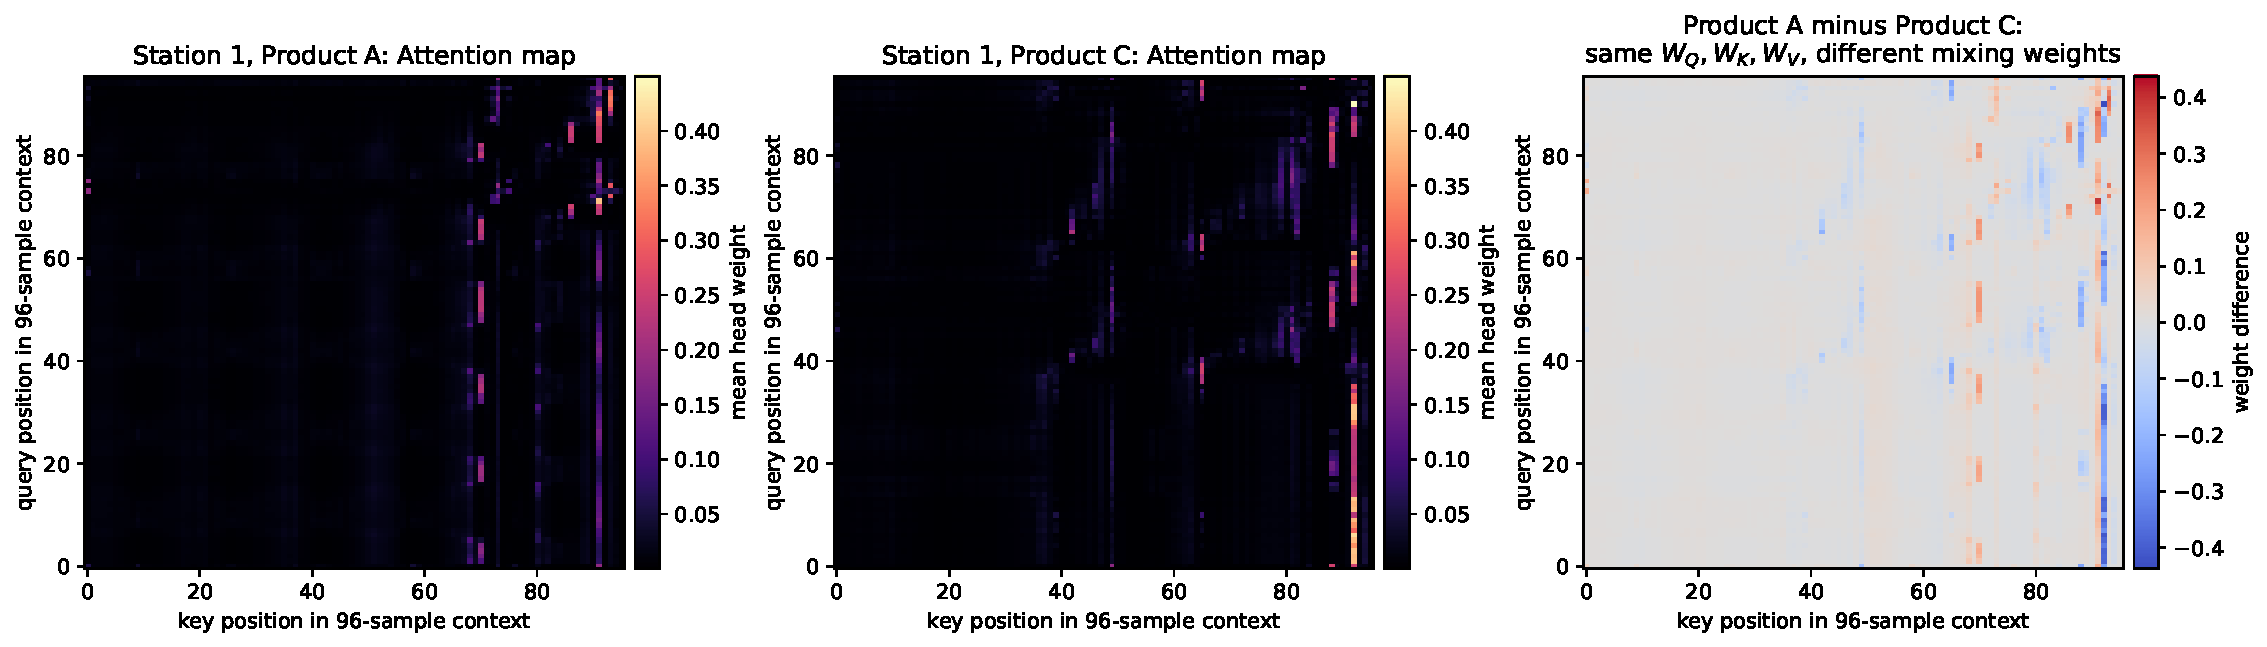
\includegraphics[width=\linewidth]{figures/task1/1.3-1.pdf}
\caption{Output 1.3: first-layer Attention (mean over heads) for the same two validation windows of station 1, and their difference.}
\end{figure}

\textbf{How the same projections produce different mixing} (station 1, validation). $W_Q, W_K, W_V$ are fixed after training, but the $96\times96$ weights $\operatorname{softmax}(QK^\top/\sqrt{d_h})$ are recomputed from each window. Both maps put their weight on the most recent 30 or so keys, but on different columns: Product~A favours keys near 70 and 90--94, while Product~C spreads weight across keys near 42, 49, 65 and 80--93. The difference map has mean $|\Delta| = 0.013$ but a maximum of 0.44, so some queries move 44\% of their weight to different positions. Because the output is $A(X)V$, each window gets its own value-mixing operator, without refitting and without a router. Ridge applies the same $\hat W$ to both windows. This figure shows only that the mixing depends on the input; it is not evidence that Attention recovered the physical period.

% ---------------------------------------------------------------------------------------------
\subsection*{Response 2 -- separating slow structure from repetition}

\begin{figure}[H]\centering
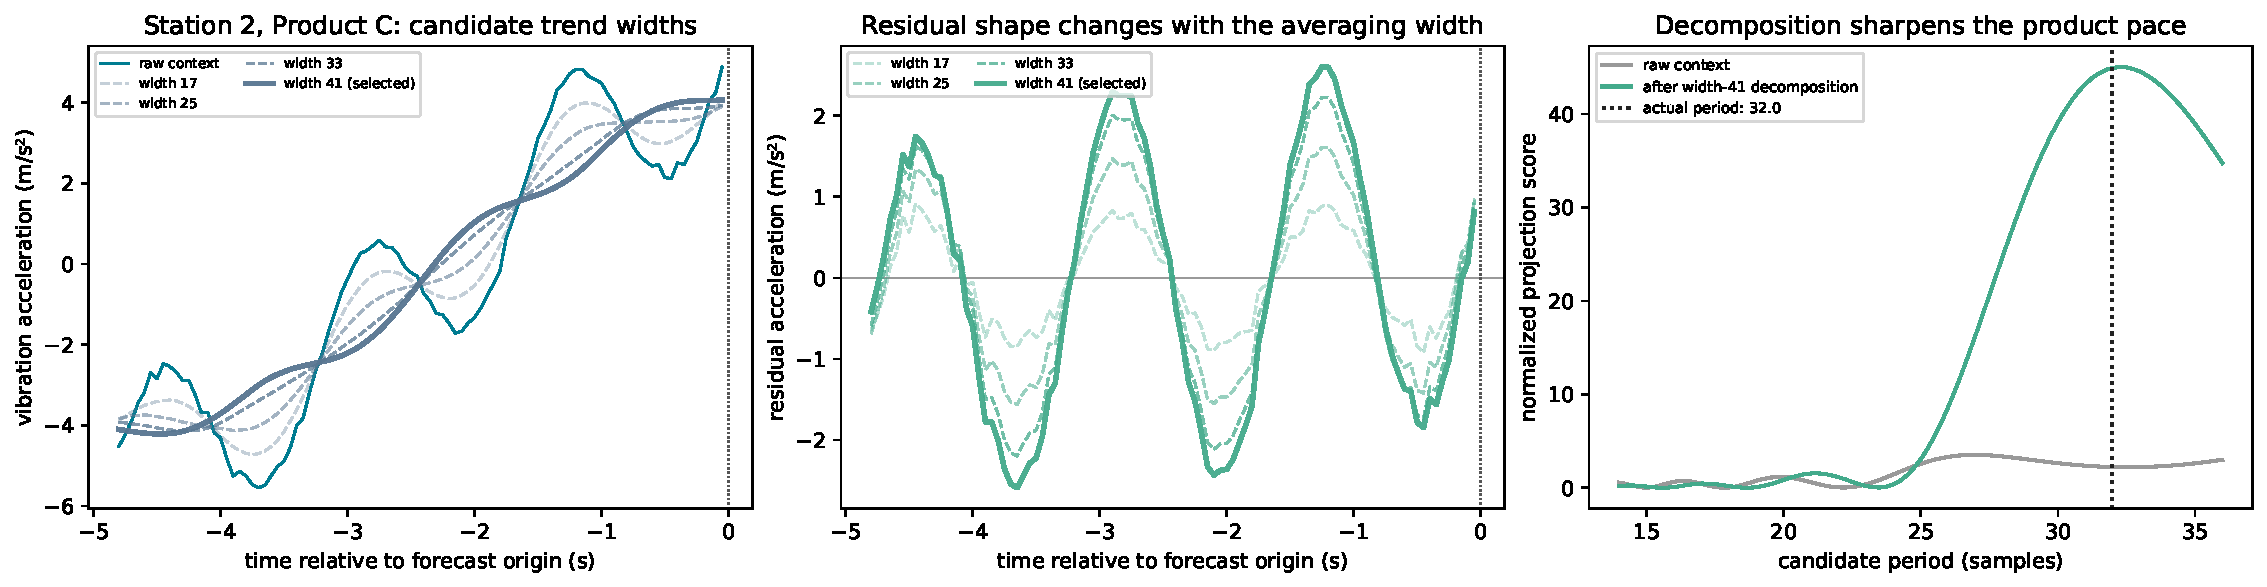
\includegraphics[width=\linewidth]{figures/task1/2.1-1.pdf}\\[2pt]
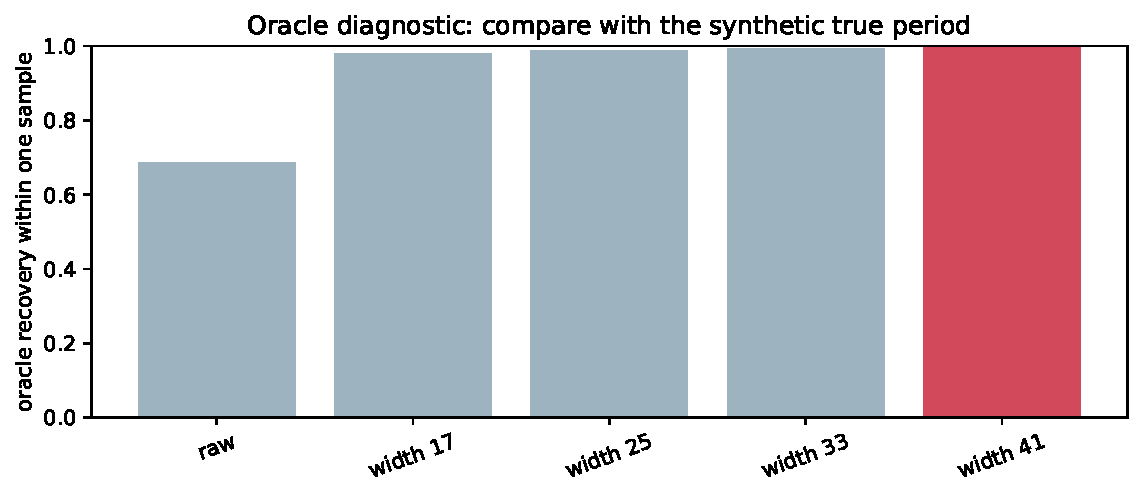
\includegraphics[width=0.55\linewidth]{figures/task1/2.2-1.pdf}
\caption{Output 2.1 (top): candidate widths on the validation window where the raw period estimate is most wrong (station 2, Product C, $P=32$). Output 2.2 (bottom): oracle period recovery on training windows of the established stations.}
\end{figure}

\textbf{Selected width and what changes.} The selected width is $m=41$.
\begin{itemize}
  \item \textbf{Output 2.1} (station 2, validation window). Narrow widths let the trend follow the vibration. At $m=17$ the trend wiggles with the 32-sample cycle, and the remainder keeps only a residual standard deviation of 0.58\ms. At $m=41$ the trend is a smooth ramp and the remainder carries the full oscillation (standard deviation 1.57\ms). The raw window's projection score has no clear peak; after the width-41 split it peaks sharply at the true period of 32.
  \item \textbf{Output 2.2} (established stations, training windows). Period recovery within one sample rises from 68.7\% on raw windows to 98.0\%, 98.9\%, 99.3\% and 99.85\% for widths 17, 25, 33 and 41.
  \item \textbf{Output 2.3} (validation). Decomposition lowers Raw Attention's RMSE from 0.408 to 0.299 on established stations ($-$27\%) and from 0.577 to 0.439 on station~4 ($-$24\%). The error falls for every product in both populations: on established stations A 0.376$\to$0.276, B 0.434$\to$0.329 and C 0.410$\to$0.289; on station~4 A 0.565$\to$0.381, B 0.548$\to$0.471 and C 0.616$\to$0.459.
  \item \textbf{Contrasting cases} (station 4, validation). In the largest-gain window, the raw model's forecast lags in phase and the decomposed model corrects it. In the smallest-gain window, decomposition slightly hurts: the forecast drifts out of phase late in the horizon.
\end{itemize}

\begin{figure}[H]\centering
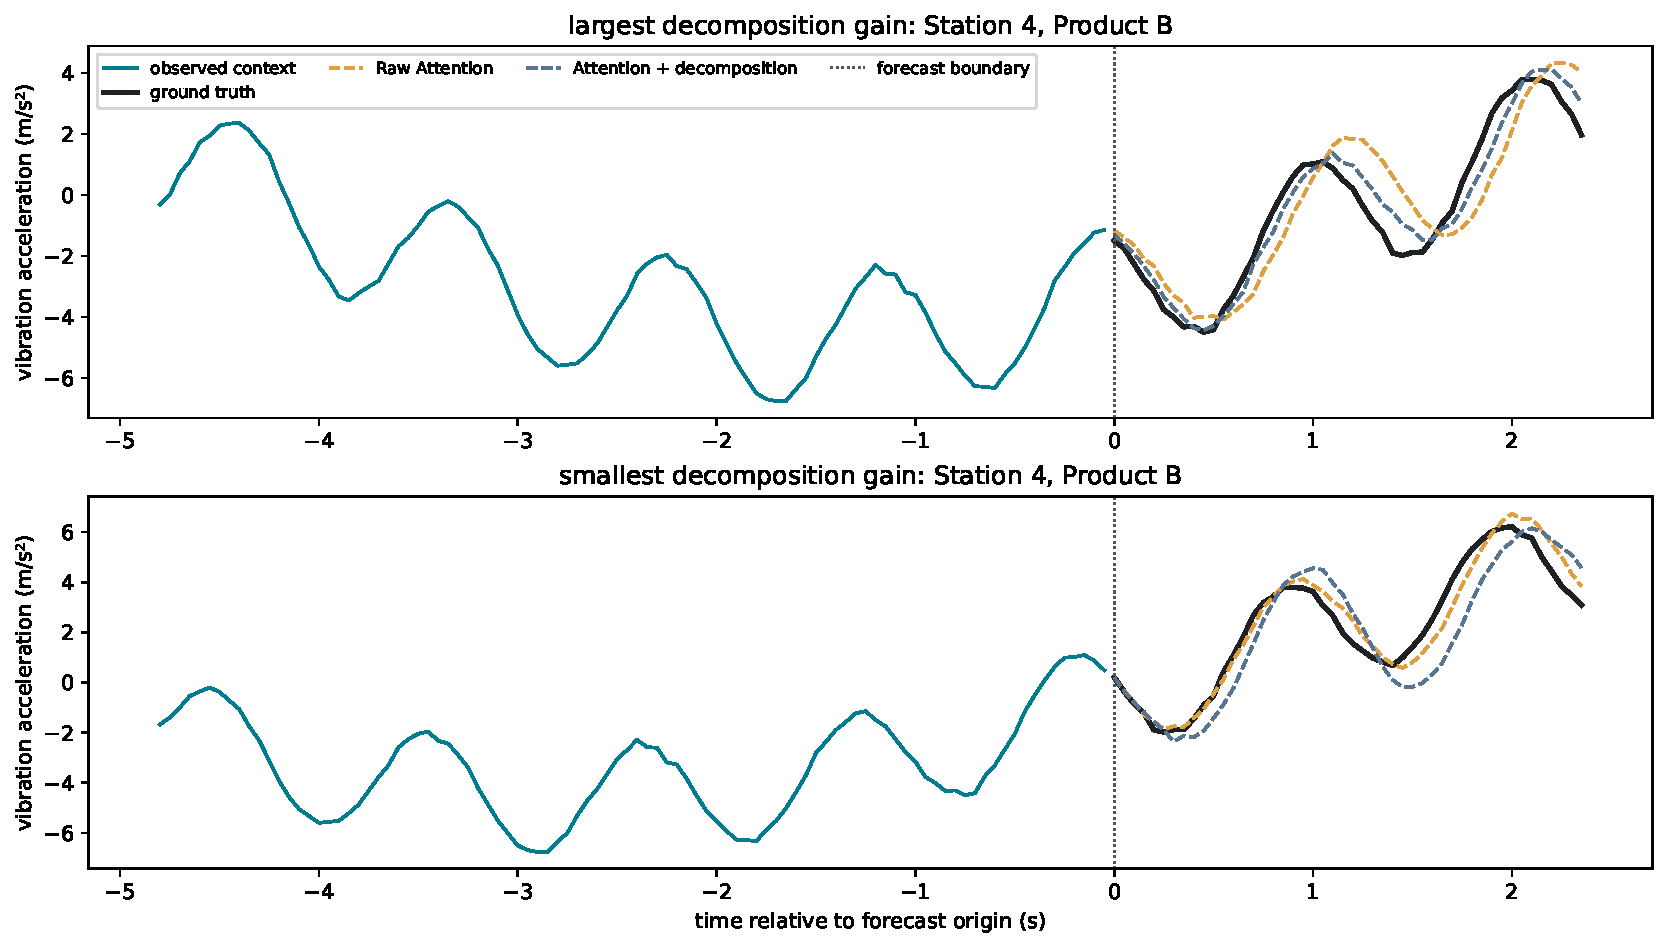
\includegraphics[width=0.8\linewidth]{figures/task1/2.3-1.pdf}
\caption{Output 2.3: validation windows with the largest and smallest decomposition gain (both on held-out station 4).}
\end{figure}

\textbf{Why a moving average suits this world.} The data are a 240-sample drift plus one 14--36-sample vibration, a wide separation of time scales. A centered average of width $m$ scales a sinusoid of period $P$ by $H(P)=\sin(\pi m/P)/(m\sin(\pi/P))$. For $m=41$ that means $H\approx0.95$ at $P=240$, while the vibration bands are attenuated to about 10--18\% on average. The drift therefore goes almost entirely to the linear trend head, and the mixer sees an almost pure oscillation. The filter has no parameters, is linear and differentiable, and introduces no phase shift.

\textbf{Why the oracle diagnostic is a good selector here.} In this simulator the true period of every window is known, so we can measure directly whether a width exposes the repetition, which is the property the mixers depend on. The measurement uses training windows from established stations only, never touches validation or test, and never feeds the true period to a model. It is also cheap, needing no training per width. A deployed system would have no true period and would need a proxy such as validation error.

\textbf{Where the bias fails.} It fails on an abrupt level shift, such as a load step. A width-41 average smears a step of height $h$ into a 41-sample ramp and leaves a $\pm h/2$ artifact in the remainder. It also fails at the context edges when the drift curves: replicate padding assumes the signal is flat beyond the edge, so at the last sample the trend lags a ramp of slope $a$ by $a\,q(q+1)/(2m)\approx5.1a$. An alternative is STL (loess-based decomposition; Cleveland et al., 1990), which fits a smooth trend robustly and handles curvature better. It encodes a known seasonal period and gives up the parameter-free, period-agnostic behaviour.

% ---------------------------------------------------------------------------------------------
\subsection*{Response 3 -- mixing by temporal delay}

\textbf{Output 3.1} confirms that the supplied FFT scores equal a direct circular correlation on $[1,3,1,3]$: $(4,-4,4,-4)$.

\textbf{Aggregation check.} My \texttt{aggregate\_delays} reproduces the notebook's worked example exactly: $z=[35,15,25,25]$ for $v=[10,20,30,40]$, delays $[1,3]$ and weights $[\tfrac34,\tfrac14]$. Since $z_0=\tfrac34 v_3+\tfrac14 v_1=35$ (not 25), position $t$ reads from $t-\tau$ as equation (6) requires. The notebook's gradient and wrap-around checks also pass.

\begin{figure}[H]\centering
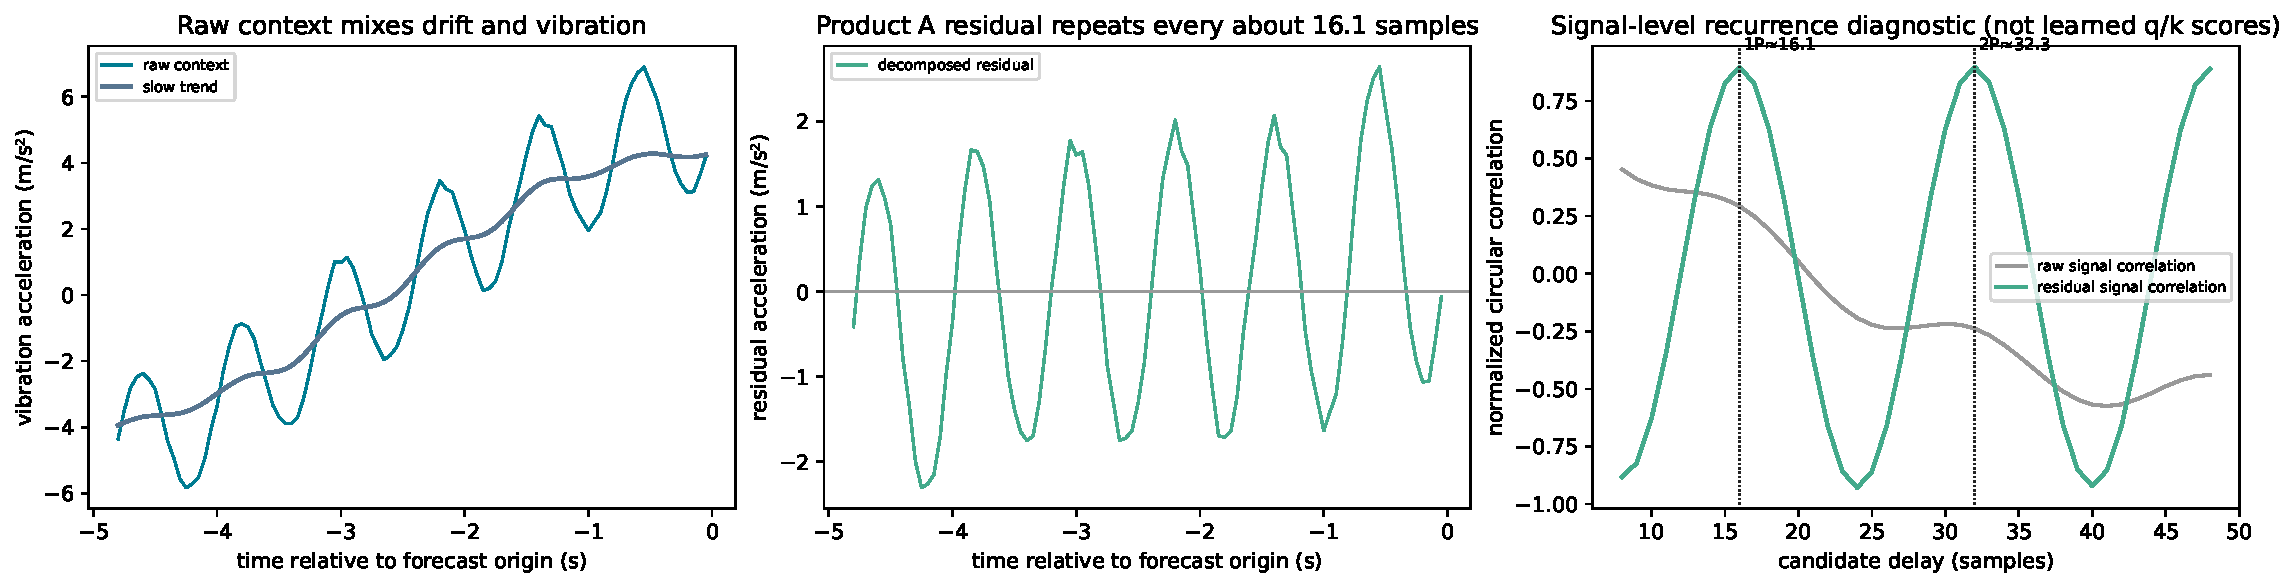
\includegraphics[width=\linewidth]{figures/task1/3.2-1.pdf}
\caption{Output 3.2: signal-level recurrence diagnostic for one validation window (station 2, Product A, $P=16.13$). These are not the model's learned q/k scores.}
\end{figure}

\textbf{Strongest lags} (station 2, validation window). The remainder's correlation peaks at delays 16 (0.896) and 32 (0.897). These are the integers nearest $P=16.13$ and $2P=32.27$. Troughs of about $-0.92$ fall near 24 and 40, the odd multiples of $P/2$, and the curve rises again toward 48, close to $3P=48.4$.

\textbf{Why decomposing first makes the evidence cleaner.} In the same window, the raw correlation declines smoothly from about 0.45 at delay 8 to about $-0.57$ near delay 41, with no peak at $P$ or $2P$. A circularly shifted ramp correlates with itself as $1-6\tau(L-\tau)/(L^2-1)$, a broad U shape, and the wrap-around seam adds a jump. Together these swamp the vibration's $\cos(2\pi\tau/P)$ pattern. Removing the trend leaves an almost pure sinusoid, so the scores in the 8--48 band concentrate on $P$ and $2P$.

\textbf{Why this supports the delay mixer.} The mixer assumes the useful relationships in a window are a few recurring displacements. It keeps the top $K$ delays, which cluster at $P$ and $2P$, and blends shifted copies, which amounts to a learned, soft seasonal-naive copy from one period back. The same bias pays off in the models: on established stations, the raw delay mixer has half the validation RMSE of Raw Attention (0.225 vs 0.408, Output 4.1).

\textbf{Where the assumption is wrong.} A pace that changes \emph{within} a context, such as run-up after a changeover or a slipping belt, breaks it. No single displacement then aligns the whole window. The top-$K$ delays become a compromise, and the blended copies are misaligned, smearing the waveform with a phase error that grows across the window. An isolated transient, such as a jam impact, also breaks it: shifting copies it $\tau$ samples later, and wrap-around places it near the start, creating ghost echoes of a one-off event.

% ---------------------------------------------------------------------------------------------
\subsection*{Response 4 -- comparing designs and deploying}

\begin{table}[H]\centering\small
\caption{Outputs 1.1 and 4.1, validation. RMSE in \ms, MSE in \mss.}
\begin{tabular}{lrrrrrr}
\toprule
 & \multicolumn{2}{c}{Established} & \multicolumn{2}{c}{Station 4} & & \\
\cmidrule(lr){2-3}\cmidrule(lr){4-5}
Model & RMSE & MSE & RMSE & MSE & Params & Fit (s) \\
\midrule
Shared ridge & 0.767 & 0.588 & 0.876 & 0.767 & 4{,}608 & 0.002\\
Sensor-specific ridge & 0.768 & 0.590 & -- & -- & 13{,}824 & 0.002\\
Period-routed ridge & \textbf{0.166} & \textbf{0.028} & \textbf{0.173} & \textbf{0.030} & 59{,}904 & 0.004\\
Raw Attention & 0.408 & 0.166 & 0.577 & 0.333 & 368{,}368 & 53.1\\
Raw delay mixer & 0.225 & 0.051 & 0.338 & 0.114 & 368{,}370 & 70.3\\
Attention + decomposition & 0.299 & 0.089 & 0.439 & 0.192 & 373{,}024 & 70.4\\
Autoformer-inspired & 0.197 & 0.039 & 0.244 & 0.059 & 373{,}026 & 74.8\\
\bottomrule
\end{tabular}
\end{table}

\begin{table}[H]\centering\small
\caption{Effect of each switch: reduction in validation RMSE (\ms); positive means the switch helps. The last column restricts established stations to the third of validation contexts with the most drift (supplementary analysis, \texttt{task1/analysis\_slow\_component.py}).}
\begin{tabular}{lrrr}
\toprule
Change & Established & Station 4 & High-drift third\\
\midrule
Decomposition, with Attention & 0.109 & 0.138 & 0.020\\
Decomposition, with delay mixing & 0.028 & 0.094 & 0.002\\
Delay mixing, raw input & 0.183 & 0.239 & 0.134\\
Delay mixing, decomposed input & 0.102 & 0.195 & 0.116\\
Both switches together & 0.211 & 0.333 & 0.136\\
Interaction (together $-$ sum of solo gains) & $-$0.081 & $-$0.044 & $-$0.018\\
\bottomrule
\end{tabular}
\end{table}

\begin{figure}[H]\centering
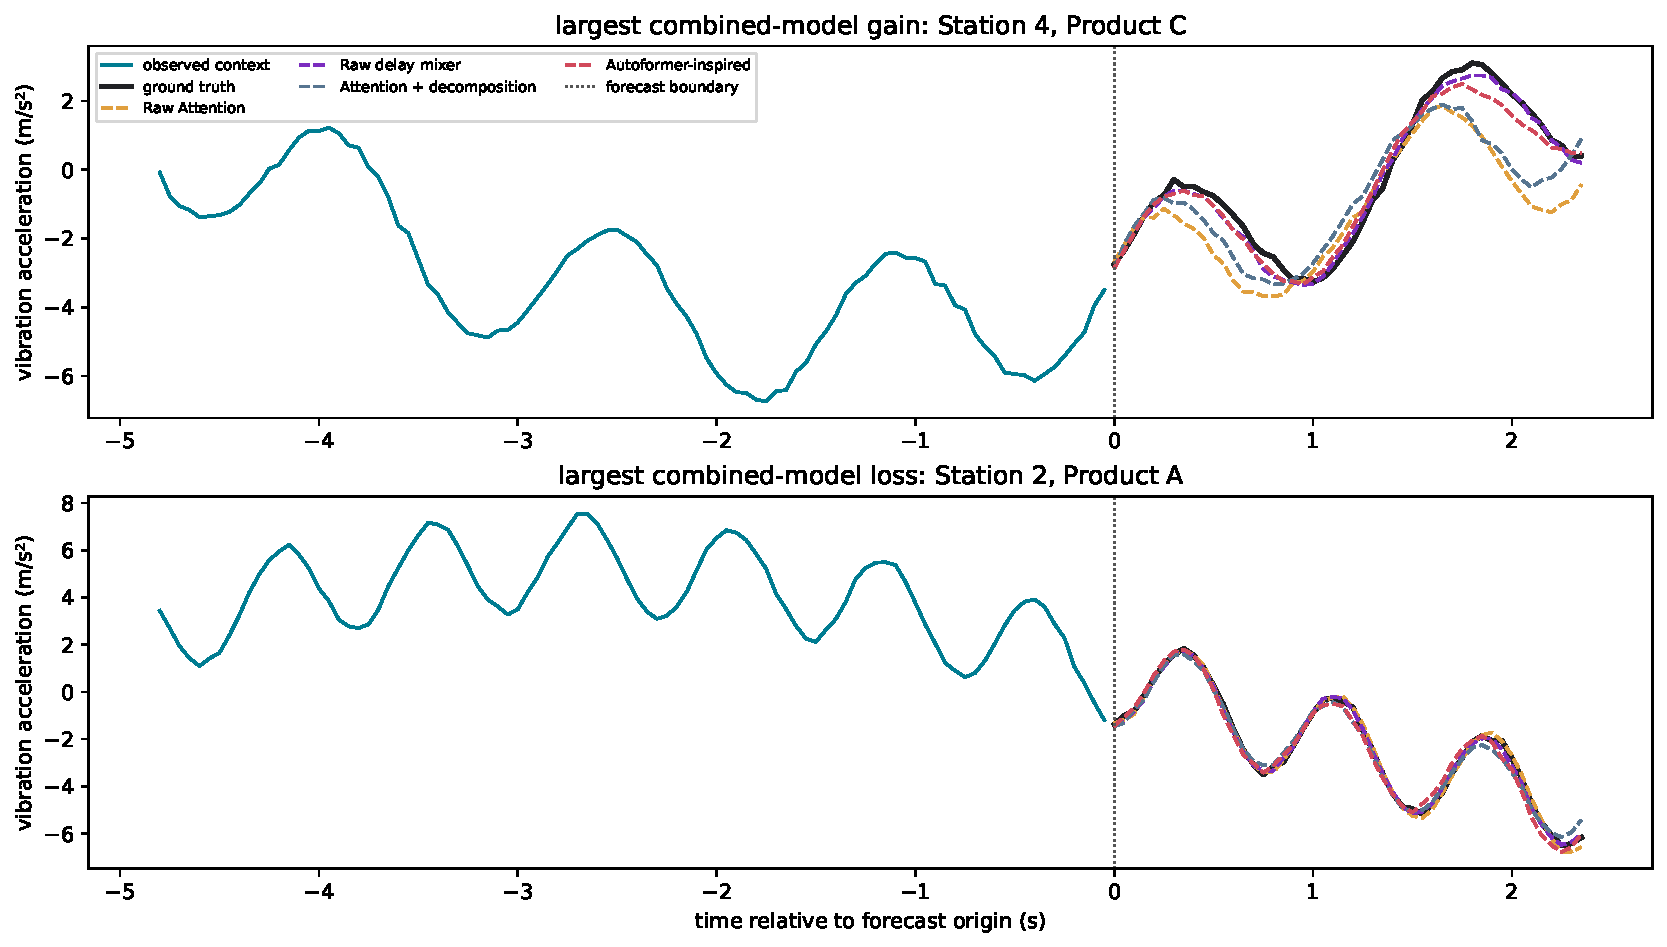
\includegraphics[width=0.75\linewidth]{figures/task1/4.1-1.pdf}
\caption{Output 4.1: validation windows with the largest gain (station 4, Product C) and largest loss (station 2, Product A) of the Autoformer-inspired model over Raw Attention.}
\end{figure}

\begin{figure}[H]\centering
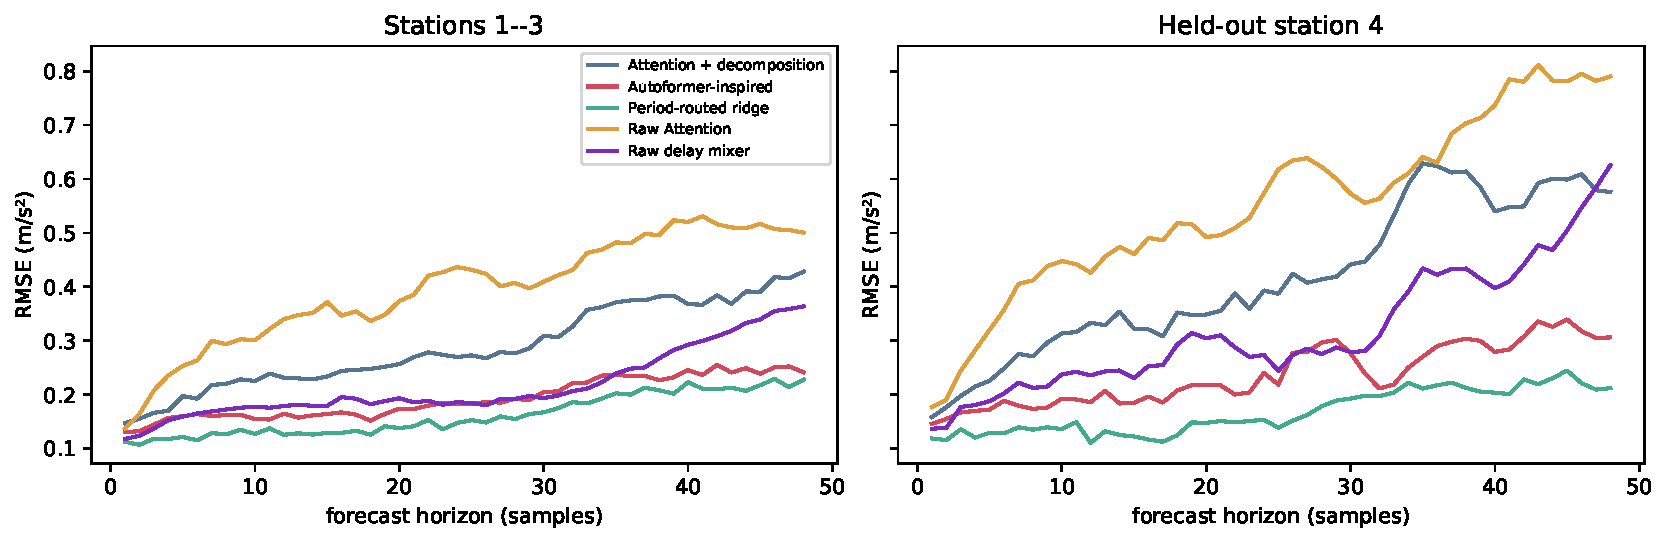
\includegraphics[width=0.85\linewidth]{figures/task1/4.2-1.pdf}
\caption{Output 4.2: validation RMSE along the 48-step horizon, established stations (left) and station 4 (right).}
\end{figure}

\textbf{(a) Prediction} (recorded before Output 4.1). Decomposition should help most on contexts where the slow component is prominent, because it removes the ramp before the mixer sees it. Delay mixing on a raw, ramp-dominated context would score delays by ramp-dominated correlations.

\textbf{(b) Evidence} (validation). On established stations, each switch helps in both settings; delay mixing is the larger in both. The gains overlap: together they gain less than their sum (interaction $-0.081$ in RMSE, $-0.065$ in MSE), and station~4 agrees. On high-drift contexts, delay mixing still gains far more than decomposition, so my prediction is not supported. Along the horizon, errors start at 0.11--0.15. By step 48, Raw Attention reaches 0.50, while routed ridge (0.23) and the Autoformer-inspired model (0.24) stay lowest in both populations.

\textbf{(c) Deployment.} I chose period-routed ridge for both populations, from validation, before Output 4.3. It has the lowest validation MSE and RMSE on established stations (0.028 / 0.166) and on station~4 (0.030 / 0.173). It uses 16\% of the neural models' parameters, fits in closed form in milliseconds, and needs no station identity. Its risk is reliance on hand-set pace bands. Its test RMSE (0.161 established, 0.183 station~4) confirms the choice.

\begin{table}[H]\centering\small
\caption{Output 4.3: the selected models on validation and test.}
\begin{tabular}{llrrrr}
\toprule
Population & Model & Val.\ MSE & Val.\ RMSE & Test MSE & Test RMSE \\
\midrule
Established & Period-routed ridge & 0.0275 & 0.166 & 0.0260 & 0.161\\
Held-out station 4 & Period-routed ridge & 0.0298 & 0.173 & 0.0333 & 0.183\\
\bottomrule
\end{tabular}
\end{table}

\paragraph{Task 1 in one sentence.} On this benchmark the right inductive bias beat flexibility: a linear map conditioned on the pace outperformed every learned design on both populations (validation), and the best neural model, the Autoformer-inspired one, approaches it only by learning a soft version of the same idea, organizing the window by its period.

\section*{Task 2 -- Autoformer leaderboard challenge}

All code is in \path{task2/src/}. Every number below is read from the JSON logs in \path{task2/results/}, except the leaderboard scores, which are copied from the leaderboard site. Unless stated otherwise, metrics are on the 18 validation blocks described in Section 2.2.

% ---------------------------------------------------------------------------------------------
\subsection*{2.1 What the data look like}

\begin{figure}[H]\centering
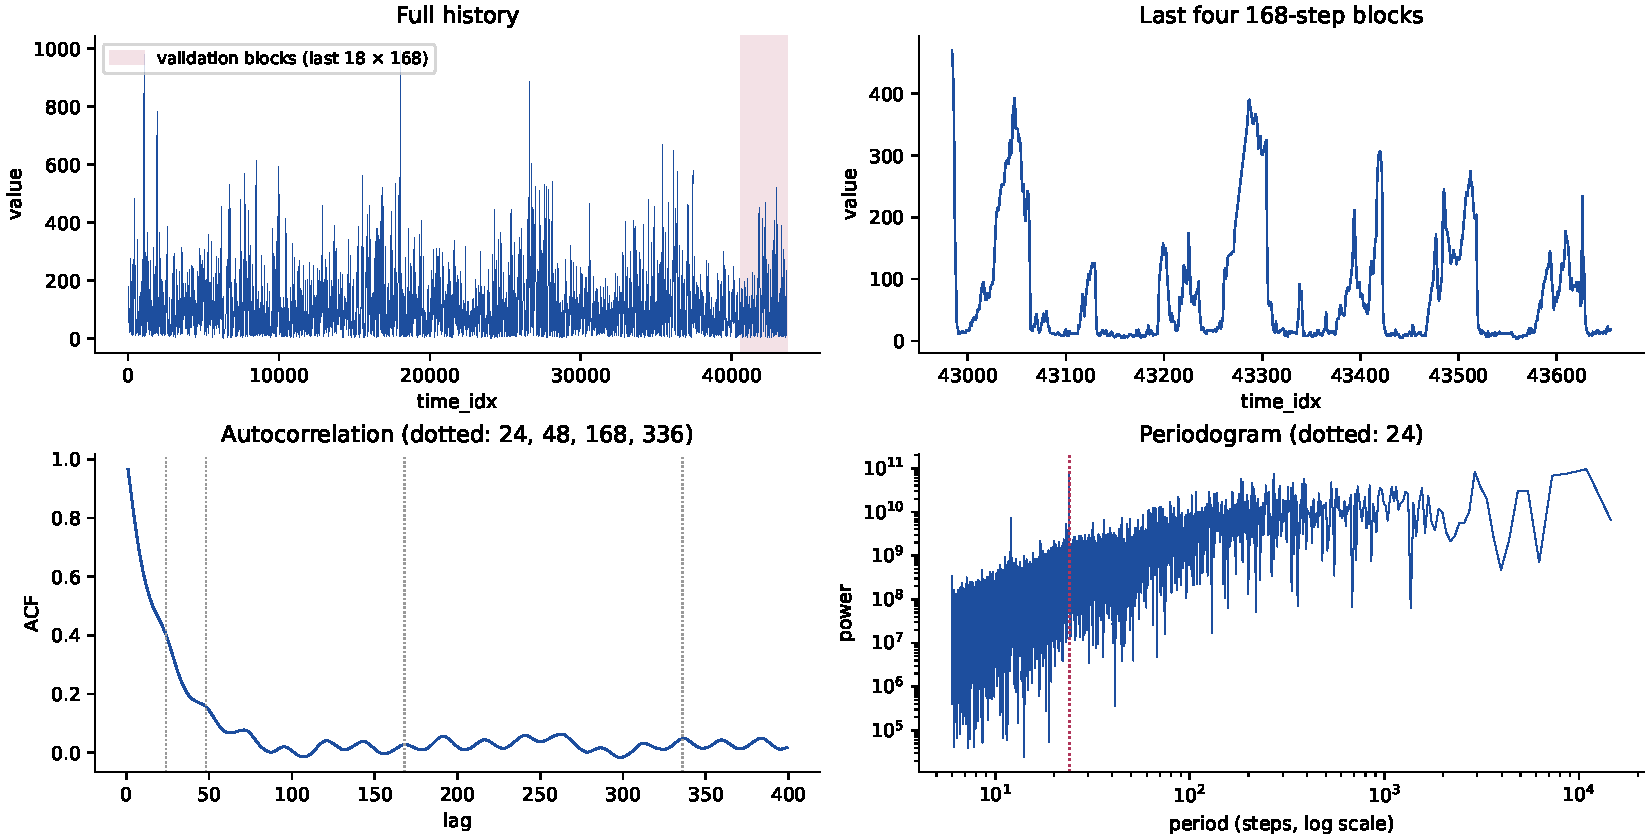
\includegraphics[width=\linewidth]{figures/task2/eda.pdf}
\caption{The target series. Top: full history (validation region shaded) and the last four 168-step blocks. Bottom: autocorrelation and periodogram.}
\end{figure}

\begin{itemize}
  \item \textbf{Target.} There are 43{,}656 integer, non-negative values with no gaps. The distribution is heavy-tailed: median 73, 99th percentile 418, maximum 994. The series builds up over several days and then collapses abruptly, which is why a single 168-step block can have a large RMSE.
  \item \textbf{Memory is short.} The autocorrelation is 0.97 at lag 1, 0.40 at lag 24, 0.16 at lag 48 and about 0.03 at lag 168. Persistence is therefore useful for a few steps only.
  \item \textbf{Periodic structure, recovered from the data.} The periodogram has one sharp line at exactly 24 steps, a small bump at 24 in the ACF, and power at very long periods (about 8{,}700--11{,}000 steps). Weekly-scale structure (168) is weak, and no single cycle dominates, as the handout warns.
  \item \textbf{External file.} It has ten variables covering all 43{,}824 steps.
  \begin{itemize}
    \item A, B and C are continuous.
    \item D, E and F are \emph{running totals that reset}. Every one of D's 8{,}283 resets coincides with a change in the categorical variable, so D accumulates while the category stays fixed.
    \item G--J are one-hot: exactly one is active at every step.
    \item The strongest same-step correlations with $\log(1+y)$ are D ($-0.35$), H ($-0.35$), A ($+0.31$) and I ($+0.23$).
  \end{itemize}
\end{itemize}

% ---------------------------------------------------------------------------------------------
\subsection*{2.2 Validation protocol and preprocessing}

\begin{itemize}
  \item \textbf{Rolling-origin validation.} The last 18 non-overlapping 168-step blocks of the history (steps 40{,}632--43{,}655) are forecast from 18 origins. Each forecast uses the true context before its origin, as a leaderboard forecast would (time-series cross-validation, Hyndman \& Athanasopoulos \S5.10).
    \begin{itemize}
      \item The \textbf{model score} is the mean over blocks of each block's RMSE, because one block is what one leaderboard submission measures. Pooled RMSE, MAE and sMAPE are logged as well.
      \item \textbf{Why 18 blocks.} A single 168-step block is a very noisy estimate for this series. The final model's per-block RMSE ranges from 28 to 107 across the 18 blocks.
    \end{itemize}
  \item \textbf{No leakage.} Training windows only have targets before step 40{,}632. Every scaling statistic is fitted on that range only.
  \item \textbf{Target transform.} The target is modelled as a z-score, either of $\log(1+y)$ or of $y$. Predictions are transformed back and clipped at zero.
  \item \textbf{Covariates.} A, B and C are z-scored. The counters D, E and F are $\log(1+\cdot)$-transformed, then z-scored. G--J stay 0/1.
  \item \textbf{Engineered covariates (final model).} Nine columns are added, all computed from the external file at every step, so they are equally available over the horizon:
    \begin{itemize}
      \item $\log(1+\Delta D)$, D's per-step increment, reconstructed by restarting the difference whenever the G--J category changes;
      \item trailing 6- and 24-step means of A, B, C and $\log(1+\Delta D)$.
    \end{itemize}
    The intuition is that the target responds to conditions accumulated over the preceding hours, not only to the current step. All statistics are fitted on the training range.
  \item \textbf{Seeds.} Every comparison uses the same seeds, blocks and windows. Results are reported as mean $\pm$ standard deviation over seeds.
\end{itemize}

% ---------------------------------------------------------------------------------------------
\subsection*{2.3 Model}

I wrote a compact Autoformer (\path{task2/src/autoformer.py}) following Wu et al.\ (2021), \S\S3.1--3.2, and the structure of the official implementation (\url{https://github.com/thuml/Autoformer}). No code was copied. It contains both defining mechanisms.

\textbf{(a) Progressive series decomposition.}
\begin{itemize}
  \item A replicate-padded moving average (kernel 25) runs after every residual sublayer in the encoder and the decoder.
  \item The encoder keeps only the seasonal part.
  \item The decoder is initialized with the seasonal and trend parts of the last \texttt{label\_len} inputs, followed by zeros and the input mean over the 168 future steps.
  \item The decoder accumulates the three trends extracted in each layer, projected by a circular \texttt{Conv1d}.
\end{itemize}

\textbf{(b) Auto-Correlation instead of dot-product attention.} This is used both for self-correlation and for encoder--decoder correlation.
\begin{itemize}
  \item It computes $R(\tau)$ for every delay with \texttt{rfft}/\texttt{irfft}.
  \item It keeps the top $k=\lfloor c\ln L\rfloor$ delays.
  \item It aggregates shifted copies of the values with softmax weights.
\end{itemize}

\textbf{Three deliberate differences from the official code.}
\begin{itemize}
  \item \textbf{External variables use the time-mark path.} The official code reserves this path for calendar features. This series has no timestamps, so an embedding of the external variables takes its place, in both the encoder and the decoder.
    \begin{itemize}
      \item In the official model this path is the \emph{only} per-step input that reaches the decoder's 168 future positions, since \texttt{forward} ignores the values of \texttt{x\_dec}. So this is where known-future information has to enter.
      \item The search started with the official per-step linear embedding. The final model uses a kernel-5 \texttt{Conv1d} with replicate padding, which gives each position a few steps of covariate context (Section 2.5).
    \end{itemize}
  \item \textbf{Delays are chosen per example} in training too, not shared across the batch.
  \item \textbf{Aggregation reads from $t-\tau$.} This matches $R(\tau)=\sum_t q_t k_{t-\tau}$ and the Task 1 convention; the official code rolls by $-\tau$.
\end{itemize}

\textbf{Anchoring (final model).} The last observed value is subtracted from the input window and added back to the output. This is Task 1's anchoring, applied here to the log-scaled target (Section 2.5).

\textbf{Training.} MSE on the transformed target, Adam, and a learning rate halved every epoch (as in the official \texttt{lradj=type1}). Every origin is used at stride 1, with a batch size of 64 and gradient clipping at 1. Early stopping uses the validation block RMSE with a patience of 2.

% ---------------------------------------------------------------------------------------------
\subsection*{2.4 Baselines and a linear probe of the external file}

Baselines calibrate what the Autoformer has to earn; only an Autoformer is submitted. Zeng et al.\ (2023) found simple linear models beating Transformer forecasters on standard benchmarks, so a linear model is the bar to clear. A direct 168-output ridge on 168 log-lags doubles as a cheap probe of \emph{which} external variables and \emph{which portions} carry signal. All numbers are validation block RMSE, MAE and sMAPE.

\begin{table}[H]\centering\small
\caption{Baselines (validation block metrics).}
\begin{tabular}{lrrr}
\toprule
Forecast & RMSE & MAE & sMAPE\\
\midrule
\inputrows{generated/baseline_rows.tex}
\end{tabular}
\end{table}

\begin{table}[H]\centering\small
\caption{Linear probe: ridge on 168 log-lags plus the listed covariate blocks (``past'' = the 24 steps before the origin, ``horizon'' = the 168 forecast steps).}
\begin{tabular}{lrrr}
\toprule
Covariates added & RMSE & MAE & sMAPE\\
\midrule
\inputrows{generated/probe_rows.tex}
\end{tabular}
\end{table}

\begin{itemize}
  \item \textbf{The value is in the horizon.} Past covariates barely help (87.3$\to$86.4). The values over the 168 forecast steps cut error by a third (87.3$\to$59.0).
  \item \textbf{Which variables.} A, B and C carry the most signal, then D and the G--J category. E and F carry none.
  \item \textbf{Target-only baselines.} None of them gets below 87.
\end{itemize}

% ---------------------------------------------------------------------------------------------
\subsection*{2.5 Model search}

\begin{table}[H]\centering\footnotesize
\caption{Every Autoformer configuration tried, in order. Values are validation block metrics, mean $\pm$ s.d.\ over seeds. The last column is the early-stopping epoch for each seed.}\label{tab:sweep}
\renewcommand{\arraystretch}{0.92}
\begin{tabular}{lrrrrl}
\toprule
Configuration & Params & Block RMSE & MAE & sMAPE & Best epochs \\
\midrule
\inputrows{generated/sweep_rows.tex}
\end{tabular}
\end{table}

What the search showed:
\begin{enumerate}
  \item \textbf{Small beats large.} Width 32 (22k parameters) overfits within one epoch. Width 16 (5.9k) is better and steadier, and width 8 (1.6--3k) is within seed noise of it. Extra encoder or decoder layers, context 96 or 336, kernel 49 and more delays ($c=3$) do not help.
  \item \textbf{Log target.} At width 16 the log and raw-scale targets tie on RMSE (65.0 vs 65.4). The log target is far better on MAE and sMAPE (45 vs 52, 54 vs 71), so I kept it.
  \item \textbf{Covariates need temporal context.} Two additions each lower error: a kernel-5 convolution in the covariate embedding, and engineered covariates (D's per-step increment, reconstructed from its resets, plus 6- and 24-step trailing means). Together they bring RMSE to 62.2 $\pm$ 3.1 over 5 seeds. The probe's advantage came from mapping covariates across time; the per-step linear embedding could not.
  \item \textbf{Anchoring.} The model largely ignored the last observation: at step 1 its RMSE was 67 against persistence's 15. Anchoring (subtracting the last value from the input window and adding it back) gives 60.8 $\pm$ 1.8. It is better on 4 of 5 paired seeds, lowers the seed spread, and makes forecasts start at the latest level.
  \item \textbf{Negative results, kept on purpose.} Replacing the decoder's \emph{mean} trend start with the last value or the end of the moving-average trend breaks the model (147--159). A start that decays from the last value to the mean also fails (71; 272 with anchoring).
    \begin{itemize}
      \item The decoder sees only the seasonal stream, so the trend start fixes the level of all 168 steps.
      \item The paper's mean start is the right bias for this mean-reverting series.
      \item The log-scale training loss rewards persistence far more than the raw-scale RMSE does.
    \end{itemize}
\end{enumerate}
Early stopping used the same 18 blocks as model selection, so the chosen configuration's validation score is somewhat optimistic.

% ---------------------------------------------------------------------------------------------
\subsection*{2.6 What the external file did (required ablation)}

The final configuration was trained under three covariate regimes. The seeds (0--4), the 18 validation blocks and every other setting are the same across arms. ``Past values only'' blanks the horizon part of the decoder's covariate input.

\begin{table}[H]\centering\small
\caption{Covariate ablation. RMSE, MAE and sMAPE are validation block metrics. The last column is the paired per-seed RMSE reduction against ``no external data'', with the number of seeds that improved.}
\resizebox{\linewidth}{!}{\begin{tabular}{lrrrrll}
\toprule
External data & Params & Block RMSE & MAE & sMAPE & RMSE per seed (0--4) & Gain vs none \\
\midrule
\inputrows{generated/ablation_rows.tex}
\end{tabular}}
\end{table}

\begin{figure}[H]\centering
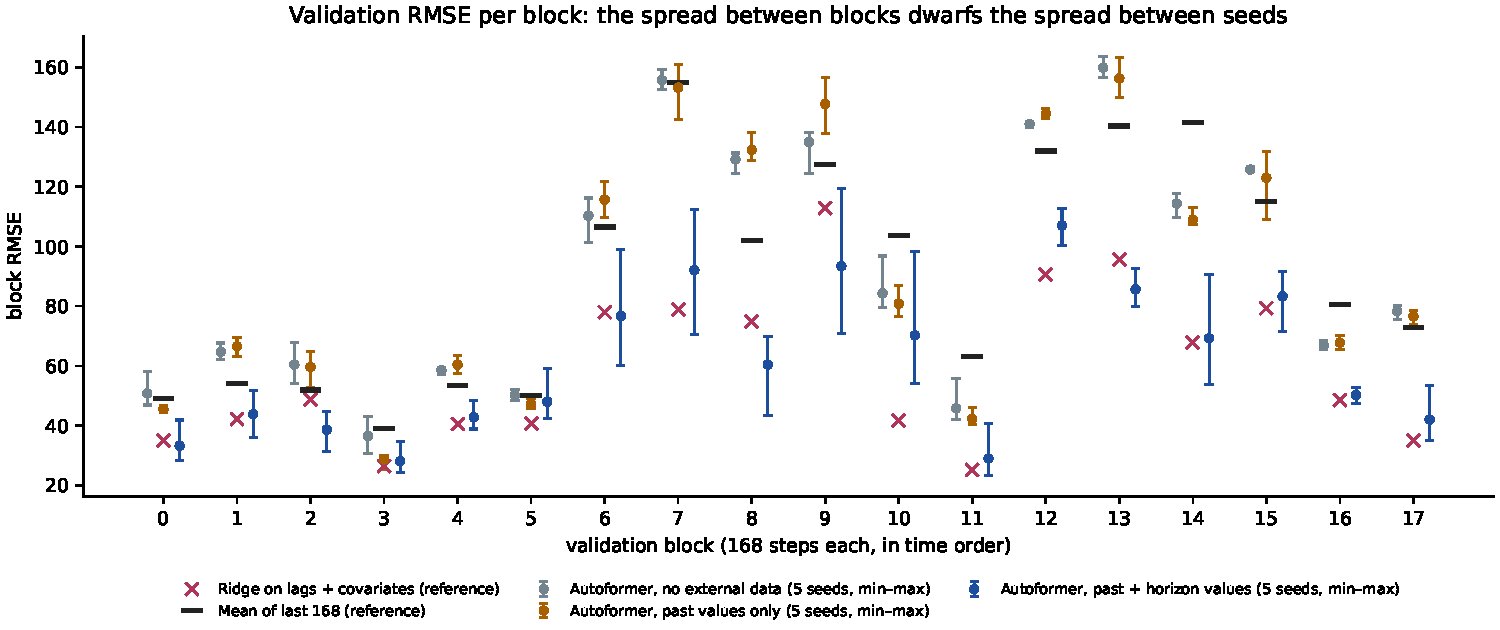
\includegraphics[width=\linewidth]{figures/task2/ablation_blocks.pdf}
\caption{Validation RMSE per block for the three arms (5 seeds, min--max bars) and two references.}
\end{figure}

\textbf{Finding.} The external file helps, and entirely through its \emph{horizon} values. With them, RMSE falls by 31.8 $\pm$ 1.6 on every seed (92.6$\to$60.8). Past values alone move it by 0.6 $\pm$ 1.8, which is within noise. This matches the linear probe.

\textbf{Why the horizon values matter.} The series builds up over days and then collapses abruptly. The future covariates indicate \emph{when} a collapse is coming (Figure~\ref{fig:weeks}). Without them, the Autoformer does no better than the naive ``mean of last 168'' baseline (92.6 vs 91.0).

\textbf{Where the values enter the model.} Known-future values can only help if they reach the decoder's 168 future positions. They do so here through the covariate embedding that replaces the official time-mark path.

\textbf{Comparison with the linear reference.} Ridge with all covariates reaches 58.1 using about 350k coefficients. The Autoformer gets within 3 points with 8.6k parameters.

\begin{figure}[H]\centering
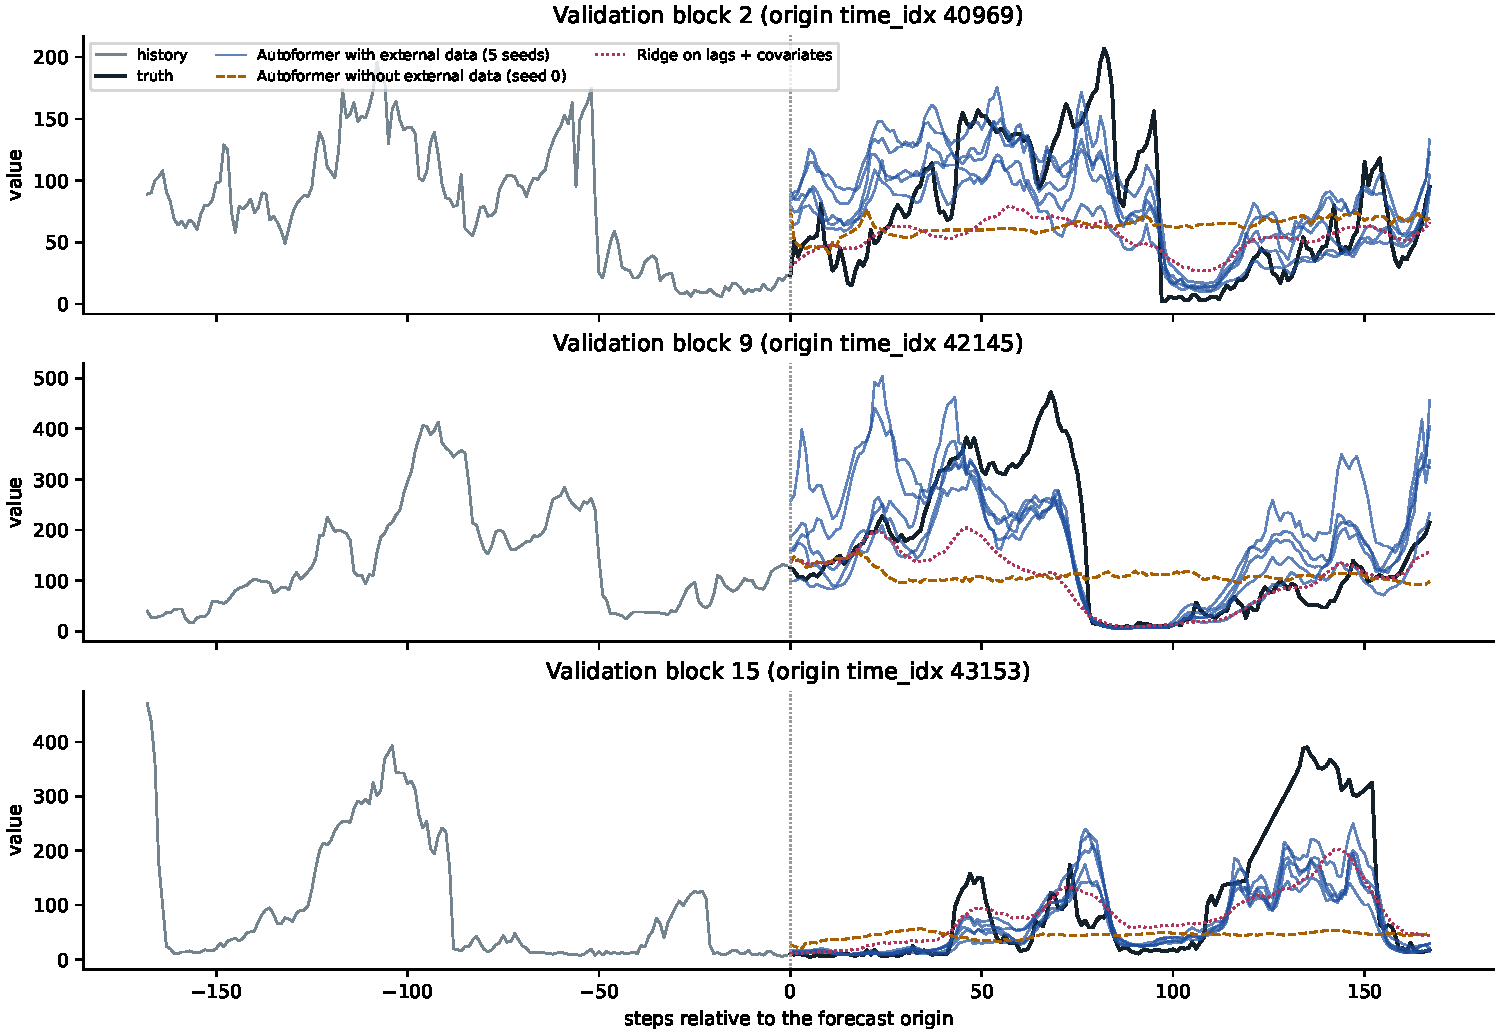
\includegraphics[width=\linewidth]{figures/task2/example_weeks.pdf}
\caption{Three validation weeks: truth, the final configuration (5 seeds), the no-covariate model, and the linear reference.}
\label{fig:weeks}
\end{figure}

% ---------------------------------------------------------------------------------------------
\subsection*{2.7 Final model, leaderboard attempts, $P$ and $E$}

\textbf{Base configuration} (shared by every submitted model). Autoformer with $d_{\text{model}}=16$, 4 heads, 1 encoder and 1 decoder layer, $d_{ff}=32$, moving-average kernel 25 and $c=1$. Context 168, label length 84, prediction length 168. Anchoring, engineered covariates with a kernel-5 covariate embedding, and horizon covariates in the decoder.

\textbf{Refit and forecast.} Each submitted model is refit on all 43{,}656 steps, with scaling refitted on all of them, for a fixed number of epochs: the median best epoch over its 5 validation seeds. It then forecasts \texttt{time\_idx} 43657--43824 (\path{task2/src/final.py}). Ensembles average the members' forecasts (\path{task2/src/ensemble.py}). As the handout requires, $P$ and $E$ are summed over members, and each member's $E$ counts both its refit epochs and the epochs its validation run spent.

\begin{table}[H]\centering\small
\caption{Leaderboard attempts on the hidden week (\texttt{time\_idx} 43657--43824). The validation column is block RMSE on the 18 validation weeks for the same model.}
\resizebox{\linewidth}{!}{\begin{tabular}{llrrrrrrr}
\toprule
Attempt & Model & $P$ & $E$ & Validation & RMSE & MAE & sMAPE & Score \\
\midrule
1 & Single log-target model (seed 0) & 8{,}577 & 6 & 57.7 & 101.10 & 61.40 & 53.79\% & 101.1060 \\
2 & Mean of 5 log-target seeds & 42{,}885 & 31 & 56.7 & 106.56 & 66.76 & 59.37\% & 106.5777 \\
\textbf{3 (counted)} & \textbf{Mean of 5 log-target + 5 raw-scale models} & \textbf{85{,}770} & \textbf{75} & \textbf{55.2} & \textbf{85.04} & \textbf{55.17} & \textbf{61.60\%} & \textbf{85.0815} \\
4 & Attempt 3 + 5 raw-loss models (15 members) & 128{,}655 & 106 & 54.4 & 89.69 & 56.93 & 60.06\% & 89.7411 \\
5 & Same forecast as attempt 4 (accidental resubmission) & 128{,}655 & 106 & 54.4 & 89.69 & 56.93 & 60.06\% & 89.7411 \\
\bottomrule
\end{tabular}}
\end{table}

\begin{figure}[H]\centering
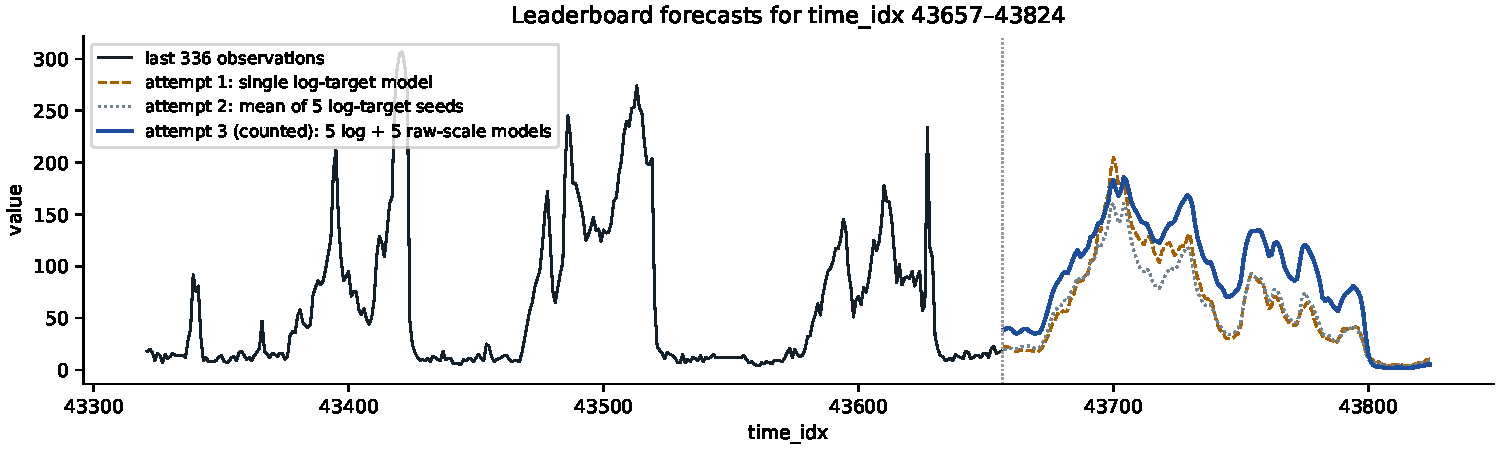
\includegraphics[width=\linewidth]{figures/task2/final_forecast.pdf}
\caption{The three leaderboard forecasts after the last 336 observations. Attempt 3 is the counted one.}
\end{figure}

\textbf{Attempts 1 and 2.} Attempt 1 scored RMSE 101.1. Most of the class scored 63--85 on the same week, so a ``hard week'' does not explain it. Attempt 2 averaged five seeds, which won on all 18 validation weeks, yet it scored worse (106.6).

\textbf{Post-mortem, done on validation only.} The two results prompted a check of the validation forecasts for systematic error, and there was one.
\begin{itemize}
  \item \textbf{The log-target model under-predicts.} Its validation forecasts average 84.8 against a true 96.6. On the busiest weeks it misses by 35--59 units and reaches only about half of the true peaks. Back-transforming a log-scale forecast gives a median-like value, below the mean of a right-skewed target. RMSE punishes this on high-level weeks, while MAE and sMAPE barely notice.
  \item \textbf{Attempt 1's forecast for the hidden week sits low.} It averages 63.8, against a long-run level of 98.
  \item \textbf{Averaging seeds kept the bias.} Attempt 2 averaged five copies of the same biased model, which only smoothed it.
  \item \textbf{A single correction factor does not fix it.} The best factor, $\times1.10$, moves validation RMSE only from 60.8 to 60.4, and fitting it on half of the weeks gives inconsistent results on the other half.
  \item \textbf{Retraining on the raw scale over-corrects.} The same configuration trained on the raw-scale target (stage 8) has a validation forecast mean of 104.3 and block RMSE 62.8.
  \item \textbf{Averaging both families cancels the bias.} The 10-member average has a validation forecast mean of 94.6, block RMSE 55.2, the best of any submission candidate, and a worst week of 94.9 against 106.4.
\end{itemize}

\textbf{Attempt 3} is that 10-member average. It scored RMSE 85.04 on the hidden week and is the counted best. It improved the rank from 37th to 31st of 40 at the time; the standing was 35th of 55 on the evening of 5 October.

The investigation was prompted by leaderboard feedback, but the model was chosen on validation evidence. The site ranks by the best attempt, not the last as the handout states.

\textbf{Attempts 4 and 5.} I then tested further variants on validation (stages 9 and 10 in Table~\ref{tab:sweep}).
\begin{itemize}
  \item Wider models and a longer context did not help.
  \item A log-target model trained with its loss on the raw scale helped only as an extra ensemble member. Adding five such models gave validation block RMSE 54.4 against 55.2, better in 10 of 18 weeks. That gain of $0.8$ has a standard error of $1.0$, so it is within noise.
  \item I submitted it anyway, because the best attempt counts and a submission therefore carries no downside. It scored 89.69, worse than attempt 3, so attempt 3 still counts.
  \item Attempt 5 is an accidental resubmission of the same forecast.
\end{itemize}
This is the clearest demonstration in this report that a validation gain inside the noise band does not carry over to a single week.

From the scores, the cost penalty is about 0.0005 per epoch, with a near-zero weight on parameters (the score minus RMSE is 0.003, 0.016, 0.038 and 0.053 for $E=6$, 31, 75 and 106).

\textbf{Declared for the counted attempt.}
\begin{itemize}
  \item $\boldsymbol{P = 85{,}770}$: 10 members of 8{,}577 trainable parameters each.
  \item $\boldsymbol{E = 75}$: the sum over members of refit epochs plus validation-run epochs. The 5 log-target members contribute 6, 5, 8, 6 and 6. The 5 raw-scale members contribute 7, 11, 7, 8 and 11 (3 refit epochs each).
  \item The forecast is in \path{task2/results/blend10_submission.txt} and the declaration in \path{blend10_declaration.json}.
\end{itemize}

\textbf{Lesson.} I first chose the log target because, at 3 seeds, it tied the raw scale on block RMSE and won clearly on MAE and sMAPE. Block RMSE alone did not expose the level bias that later cost the most on the leaderboard. Checking whether the mean forecast matches the mean truth would have caught it before the first submission.

% ---------------------------------------------------------------------------------------------
\subsection*{2.8 Where the three metrics disagree}

\begin{itemize}
  \item \textbf{Log vs raw-scale target.} Training on the log target instead of the raw scale leaves RMSE unchanged (65.0 vs 65.4). It improves MAE by 13\% and sMAPE by 24\%. Back-transforming a log-scale mean gives a median-like forecast, which MAE and sMAPE reward. RMSE, dominated by the spikes, is indifferent.
  \item \textbf{Persistence vs seasonal naive.} The metrics rank them in opposite orders. Persistence is worse than seasonal naive at lag 24 on RMSE (135.2 vs 123.4) but better on sMAPE (93.7 vs 99.3). Copying yesterday's spikes into the wrong hours is punished heavily by a relative metric.
  \item \textbf{Pooled vs per-block RMSE.} Pooled RMSE weights the few high-level weeks more heavily, which is why it exceeds the mean per-block RMSE, for example 98.2 vs 91.0 for the mean of the last 168.
\end{itemize}
Leaderboard ranking uses RMSE, so model choices were made on block RMSE; MAE and sMAPE served as tie-breakers.

% ---------------------------------------------------------------------------------------------
\subsection*{2.9 Reflections grounded in these experiments (optional questions)}

\begin{itemize}
  \item \textbf{Q2.7 (known-past vs known-future covariates).} Here availability decides \emph{both} where a variable enters and how much it helps. The same file gives $-0.6$ RMSE through the encoder and $-31.8$ when its horizon values reach the decoder's future positions. A covariate that only describes current conditions, like the ones here, is useless if known only up to the origin, and powerful if known across the horizon.
  \item \textbf{Q2.6 (window-relative normalization).} Anchoring removes the window's level, which is exactly what the model should adapt to at short horizons. The level still matters at long horizons, and the mean trend start supplies it; replacing that start with the last value (Section 2.5) shows what is lost without it.
  \item \textbf{Q2.8 (no calendar).} The 24-step cycle was recovered from the periodogram without timestamps. Trusting it requires stationarity of that cycle, and here its ACF bump is small, so the model leans on covariates instead.
  \item \textbf{Q2.2 and Q2.3 (fixed-kernel, repeated decomposition).} Abrupt collapses are level shifts, which a kernel-25 average smears. That is one reason the covariates, not the decomposition, carry the timing of drops.
\end{itemize}


\section*{References and software}
\begin{enumerate}[label={[\arabic*]},leftmargin=2.2em]
  \item H.~Wu, J.~Xu, J.~Wang and M.~Long. Autoformer: Decomposition Transformers with Auto-Correlation for Long-Term Series Forecasting. \emph{NeurIPS}, 2021, \S\S3.1--3.2.
  \item Official Autoformer implementation, \url{https://github.com/thuml/Autoformer}. Its structure was consulted (\path{models/Autoformer.py}, \path{layers/AutoCorrelation.py}, \path{layers/Autoformer_EncDec.py}, \path{layers/Embed.py}); no code was copied.
  \item A.~Vaswani et al. Attention Is All You Need. \emph{NeurIPS}, 2017.
  \item A.~Zeng, M.~Chen, L.~Zhang and Q.~Xu. Are Transformers Effective for Time Series Forecasting? \emph{AAAI}, 2023.
  \item R.~J.~Hyndman and G.~Athanasopoulos. \emph{Forecasting: Principles and Practice}, 3rd ed., OTexts, 2021 (\S5.10, time-series cross-validation).
  \item R.~B.~Cleveland, W.~S.~Cleveland, J.~E.~McRae and I.~Terpenning. STL: A Seasonal-Trend Decomposition Procedure Based on Loess. \emph{Journal of Official Statistics}, 6(1), 1990.
  \item AI651 Assignment 1 handout, notebook and harness (Dr Momin Uppal, LUMS, Fall 2026). The three implementation cells are mine; everything else in \path{task1/harness/} and the notebook is supplied.
  \item Software: PyTorch 2.5 (Paszke et al., \emph{NeurIPS} 2019), NumPy, pandas, Matplotlib, nbclient and JupyterLab. The report was compiled with Tectonic.
\end{enumerate}

\section*{Appendix -- use of generative AI}

As the course policy requires, this appendix records the prompts, what the AI produced, and what I changed. The
tool was Claude (Anthropic), used through Claude Code with access to my assignment folder, between 25 September and 5 October 2026. The running log is in \path{AI_USAGE.md} in the repository.

\begin{enumerate}
  \item \textbf{Prompt:} ``Go through the assignment resources and prepare the 5 iteration study guide to prepare me to attempt this assignment \ldots\ teach me about the background knowledge required \ldots\ give me an estimate on how long will this assignment take?''\\
  \textbf{Output:} A five-part interactive study guide with practice notebooks on forecasting setup, Attention, moving-average decomposition, delay mixing and Autoformer, plus a time estimate.\\
  \textbf{Use:} Study material only; nothing from it is submitted.

  \item \textbf{Prompt:} ``Lets proceed with attempting the actual assignment \ldots\ we can develop the plan and work on it \ldots\ do as you think is the best \ldots\ I'll learn once we've completed the assignment.''\\
  \textbf{Output:} Everything below was produced by the AI in response to this prompt.
  \begin{itemize}
    \item \emph{Task 1:} the Response 1A and 4(a) predictions, written before any cell ran (\path{task1/predictions_before_running.md}); the three notebook implementations; a headless notebook runner; the full-preset run; the deployment choices, made from the validation summary before Output 4.3; a supplementary validation-only analysis; and drafts of Responses 1A--4.
    \item \emph{Task 2:} exploratory analysis; a compact Autoformer written from the paper and the official repository's structure; a leakage-safe rolling-origin validation; baselines; a linear covariate probe; seven stages of seeded experiments, including the negative results; the covariate ablation; the final refit and forecast.
    \item \emph{Report:} this LaTeX report.
  \end{itemize}

  \item \textbf{Prompts:} the leaderboard results of attempt 1, and later of attempt 2, pasted from the leaderboard site.\\
  \textbf{Output:} The AI updated the report. After attempt 1 showed the size and epoch penalty was tiny, it checked on the validation blocks that averaging five seeds helps, and prepared that forecast (\path{task2/src/ensemble.py}). It recommended stopping after two attempts.\\
  \textbf{Use:} I submitted both attempts myself. Attempt 1 remains the counted best.

  \item \textbf{Prompt:} ``please review the assignment document and submission and make sure nothing is incomplete \ldots''\\
  \textbf{Output:} A requirement-by-requirement review against the handout, which led to five changes:
  \begin{itemize}
    \item station-4 per-product results added to Response 1A;
    \item population and split named for every claim;
    \item Response 4 brought within 200 words, with the numbers moved into tables;
    \item an explicit worked-example check in Response 3;
    \item the Task 2 model description updated, and a references section added.
  \end{itemize}

  \textbf{My edits:} I reviewed everything and made no changes.
\end{enumerate}

\textbf{How the AI's work was verified.} The notebook's own checks passed for all three implementations, and the worked examples reproduce $[35,15,25,25]$ and the expected trend. Every number in this report is read from the executed notebook, its exported CSV files, the JSON logs in \path{task2/results/}, or the leaderboard site.


\end{document}
